\documentclass[titlepage, a4paper, 11pt]{scrartcl}

%too much whitespace otherwise
\usepackage[left=35mm,top=26mm,right=26mm,bottom=15mm]{geometry}

% deutsche Übersetzungen
%\usepackage[ngerman]{babel}
% Grafik Pakete
\usepackage{graphicx,hyperref,amssymb}
% Ordner für Grafiken
\graphicspath{ {./images/} }
% Pakete für Formatierung der Grafiken
\usepackage{wrapfig}
\usepackage{float}
% deutsches Encoding (Umlaute)
\usepackage[utf8]{inputenc}
% für Grad Symbol
\usepackage{textcomp}

% Header and Footer
\usepackage{fancyhdr}

\usepackage{titlesec}

%image grid
\usepackage{graphicx}
\usepackage{subfig}

\usepackage{multicol}

\usepackage{cite}

\usepackage{amsmath}

%\geometry{top=20mm}
\usepackage{etoolbox}

\usepackage{hyperref}
\usepackage{cleveref}

\pagestyle{fancy}
\fancyhf{}
\rhead{Lückert, Neudecker}
\lhead{Kalman filtering with collision detection}
 
\begin{document}

    \title{Kalman filtering with collision detection using the example of billiards}
    \author{Marlon Lückert \\ Bachelor of Science \\ \href{mailto:marlon.lueckert@haw-hamburg.de}{marlon.lueckert@haw-hamburg.de} 
    \and Julius Neudecker \\ Bachelor of Science \\ \href{mailto:julius.neudecker@haw-hamburg.de}{julius.neudecker@haw-hamburg.de} }
    \date{June 2020}
    \maketitle

    \tableofcontents

\begin{abstract}
In this article we are going to discuss enhancements to the Kalman filter \cite{kalman} which improve the tracking and prediction of moving objects
that may collide with other objects resulting in an abrupt change of their direction.
To illustrate and test the improvements, we use a game of billiards and track and predict the position of a moving billiard ball which collides with the cushions of the billiard table.
We developed two improved versions to the standardized Kalman filter.
The first implementation dynamically adjusts the process noise at a collision.
The second implementation takes the rebound angle into account when colliding with an object. 
The implementations were tested in a virtual simulated environment and with real world video footage of a billiard game.
We conclude this paper with a performance evaluation of the implementation and provide a proposal to further increase accuracy.
\end{abstract}


\section{Introduction}

\subsection{Kalman filter}

Kalman filtering is used to produce estimations of unknown variables based on a series of measurements over time.
It filters statistical noise and other inaccuracies by comparing the measurement with a prediction based on a previous measurement.
In order to make these predictions the observed object has to follow a linear physical model, like a moving car or a rolling ball, which enables a precise calculation of future states.
The filter cannot react to sudden changes that are caused by the environment or other objects, like the collision of a rolling ball with another object.
The Kalman filter has to be modified to receive better results in the mentioned circumstances.

\subsection{Game of billiards} \label{intro}

Billiards is perfect example of the combination of linear movement and sudden changes caused by the environment.
Linear movement happens when the ball is freely rolling. It moves with an almost constant velocity in one direction, caused by the very small rolling resistance between the material of the ball and the table.
This behavior is very suitable for the usage of Kalman filter especially when dealing with noised data.

In video analysis of billiard or snooker games the state of the art solution for tracking are computer vision algorithms \cite[p.~226]{fraenti2014structural}.
These algorithms generate noised data because they depend on the quality of the video footage, which includes the resolution, lighting conditions and perspective distortion.
The Kalman filter helps to improve the overall quality of the tracking when using visual tracking algorithms.

The problem is, when two balls hit each other or a cushion the velocity vector changes its orientation instantly. 
If this isn't taken into account, the filter needs some time to adapt to the new direction of movement and will produce wrong estimations during this time.
A kalman filter will assume the direction of movement on any given sample is about the same as in the last sample. 
It will therefore create wrong estimations if the direction of movement changes drastically in a short period of time. The time the filter needs to recover depends on the filter gain.
At this point our research begins, where we customize the filter implementation in the way that we receive good estimation even when this sudden changes of movement happen.

Additionally we not just want to improve the tracking but furthermore improve the prediction of the ball position by feeding back its estimations as actual state. 
The quality of this prediction however depends on several factors, which we discuss in detail in \cref{implementation}.

\section{Methodology}

To evaluate the performance of the different filter implementations we have to compare the filter result with the actual position of the ball.
The key figure for this comparison is the mean square error (mse), which calculates the mean value of all quadratic difference between the filtered position and the real position over a specific time frame.
We calculate the mse for the current position of the ball and the predicted future positions of the ball.
\subsection{Simulation}

To be able to calculate the mse we have to know the ground truth position of the billiard ball.
Therefore we created an environment which gives us full control of all parameters of a billiard game.
In the simulations we generate a virtual billiard game where we can set the speed of the ball, the noise of the sensor and the sampling rate of the sensor.
The simulation gives us access to all parameters of the ball and the environment these include the current position and speed of the ball and the position of the cushions of the billiard table.

\subsection{Real video footage}

Besides the evaluation with the simulation we want to test the filter implementations in real video content.
In order to create input data for the Kalman filter we have to track the balls on the billiard table. 
To provide consistent and reproducible results, we used video footage and processed it with the Python implementation of openCV.
A video example as seen in \cref{pic:pool-color} is put into an instance of simple video-processing steps to create a black and white mask of the ball contours as displayed in \cref{pic:pool-bw},
where the center of the white pixel cluster is the ball we are looking for.

\begin{figure}[H]
    \centering
    \fbox{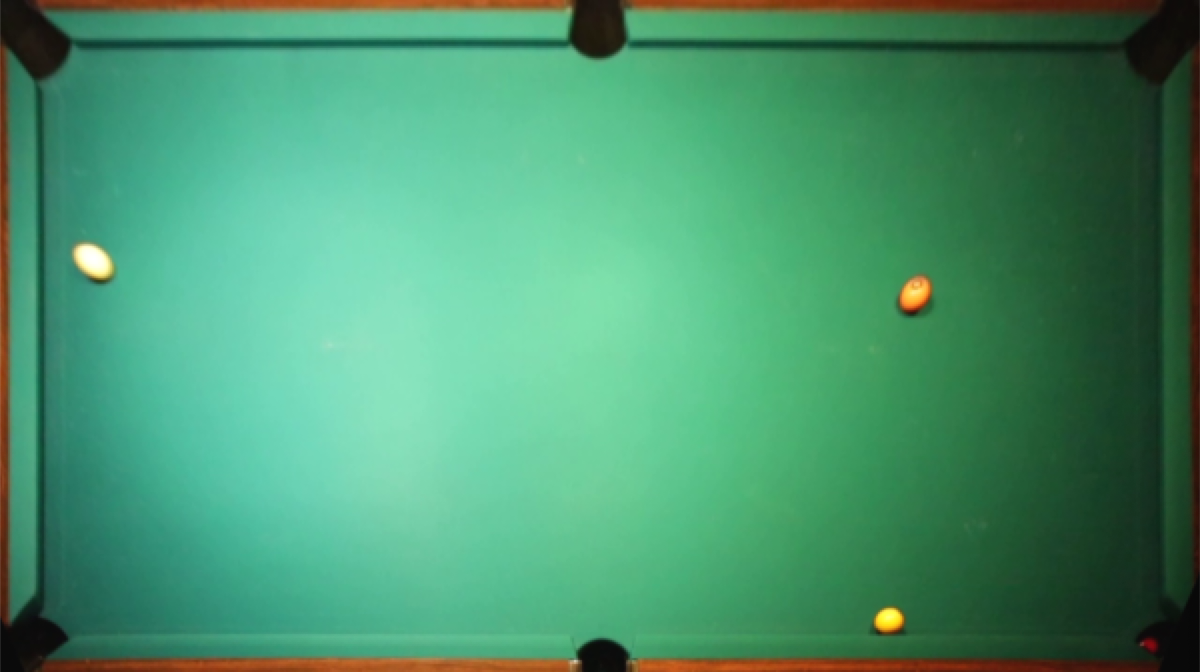
\includegraphics[width=0.68\textwidth]{pool_color.PNG}}
    \caption{color picture of a billiard table}
    \label{pic:pool-color}
\end{figure}

\begin{figure}[H]
    \centering
    \fbox{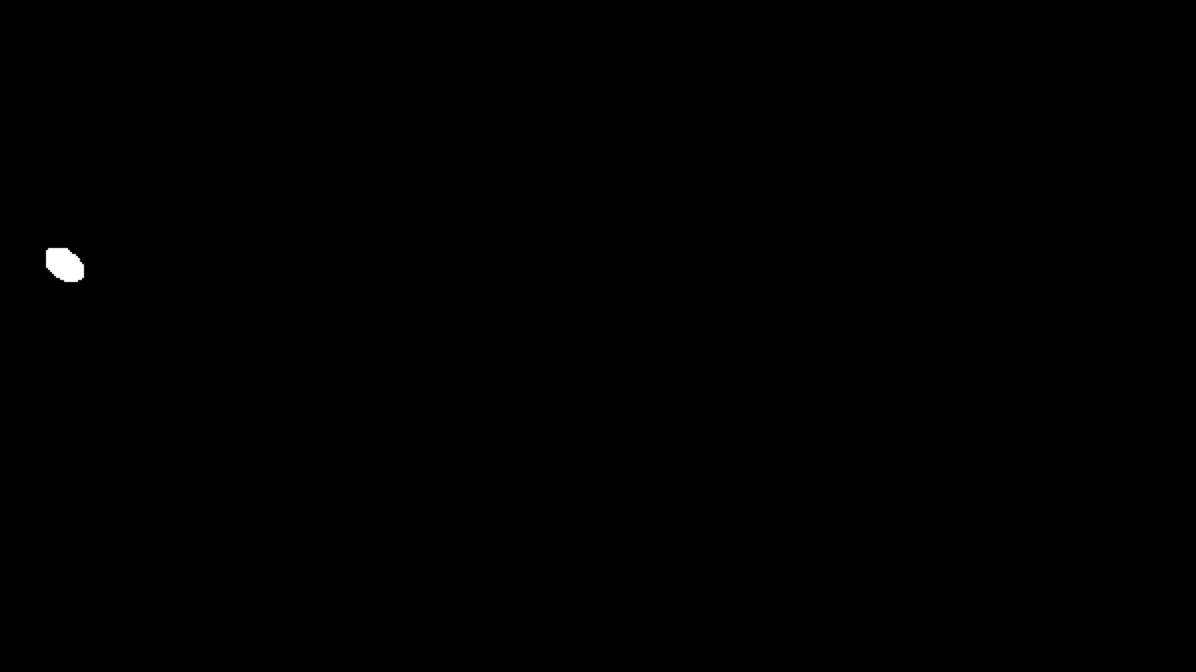
\includegraphics[width=0.68\textwidth]{pool_mask.PNG}}
    \caption{contours of balls after processing}
    \label{pic:pool-bw}
\end{figure}

In the real video footage we cannot calculate a mse for the current position. because we do not know the ground truth position just the sensor data.
But we can evaluate the prediction by comparing the predicted position to the filtered position and use this mse.

\section{Related Work}

In this section, we are going to discuss some previous work that is related to our work but none of these articles targets the problem in the same manner.

Jong-Yun Kim and Tae-Yong Kim \cite{kim} developed a method to provide robust tracking of a soccer ball. 
They provide a solution for the problem for the case that the soccer ball might be occluded by the player at any given time,
which results in a diminished tracking accuracy. 
In this case they used the velocity vector of the player to substitute for the ball presuming that the ball moves in the same direction as the player does.

Jia et.al. \cite{jia} conducted research in the trajectory of pool balls, which helped us to decide which kalman model is the most suitable.

Shiuh et.al. \cite{shiuh} provided a good starting point how to create a tracking algorithm for pool balls. They also developed an algorithm to track occluded objects using an adaptive kalman filter.
In this case they used to threshold in order to determine whether the object can still be reliably tracked. If this isn't the case the filter will rely only on predicted values until the object can be tracked reliably again.

Salzmann and Urtasun \cite{salzmann} proposed a more general approach for tracking. 
They were able to recreate a highly accurate tracking from a noisy picture based on newtons 2nd law and markov models.
Using different constraints and presumptions they were even able to extract physical parameters like friction and trajectories.

Mohamed and Schwarz \cite{schwarz} are using partly the same approach as we do to improve the results created by INS/GPS\footnote{Inertial Navigation System / Global Positioning System} Systems.
However their approach only targets the 'Q' and 'R' parameters of the filter.

Sarkka and Nummenmaa \cite{sarkka} created an adaptive kalman implementation which adapts itself to time-varying noise parameters. 
Since our filter only has two states, we decided to simulate for the optimal filter parametrization instead of relying on the filter to adapt itself.

Gabdulkhakova and Kropatsch \cite{kropatsch} use a kalman filter to create a video analysis tool for snooker game broadcasting.
They were able to show how to track snooker balls with non-linear motion.

\section{Implementation} \label{implementation}
In this section we're going to discuss the different implementations and their constraints. The filter implementations in section Dynamic-Q Filter and Smart Filter are derived from
the basic implementation in \cref{kalman-basic}. At the end of this section we will provide a comparison of all filter types and their performance in our simulation.

\subsection{Kalman Filter} \label{kalman-basic}

The basic layout and working mechanism of a kalman filter is in described in detail in \cite{kalman}. 
However in order to fully understand our improvements we provide an introduction to the crucial parts of the kalman filter.

Its purpose is to filter noisy or unreliable sensor data. 
Its doing this by comparing predictions based on the physical model and the sensor data. 
Depending on the filter gain it will use a bigger portion of either. 
This estimated value represents the actual state of the measured system and is used for the new estimate.

This is represented in \cref{eq1}

\begin{equation} 
    \label{eq1}
    \hat{x}[n]=\tilde{x}[n]+K\cdot(y[n]-C\cdot\tilde{x}[n])
\end{equation}

Where $K$ represents a matrix, which determines the amount of measured values applied to the prediction to create a new estimation. It is defined as in \cref{eq2}, 
where $\tilde{P}[n]$ is the prediction error of the current prediction, $C^T$ is a matrix to map our state vector to our measurement-model and $S$ represents the covariance matrix of the residual.

\begin{equation} 
    \label{eq2}
    K=\tilde{P}[n]\cdot C^T+S^{-1}
\end{equation}

Every prediction which is used in \cref{eq1}, was previously calculated using the state transition model $A_d$:

\begin{equation} 
    \label{eq3}
    \tilde{x}[n]=A_d\cdot\hat{x}[n-1]
\end{equation}

The state transition matrix $Ad$ defines the motion model of our filter.
We are going to use the constant velocity model, because the ball is rolling straight without any curves.
The estimation error $\tilde{P}[n]$ is defined in \cref{eq4}:

\begin{equation} 
    \label{eq4}
    \tilde{P}[n]=A_d\cdot\hat{P}[n-1]\cdot A_d^T+G_d\cdot Q\cdot G_d^T
\end{equation}

The element $Q$ is the important part here. It defines the amount of process noise in the whole filter process, which we are going to discuss in \cref{dynamic-q}.

\subsection{Dynamic-Q Filter} \label{dynamic-q}

We previously mentioned in \cref{intro}, that depending on the model the filter can't adapt to sudden changes in direction of the moving object. 
The case where the ball collides with the cushion can be mitigated by choosing a different values for $Q$ in \cref{eq4} within the crucial time window.
Thus the filter relies more on the measurement than the estimations. By doing so it can adapt momentarily.
We implemented a look-up table and constantly check every sample for proximity to a cushion.

We have to feed the filter with two additional parameters: The position of the cushion and the dynamic q-parameter.

In order to parametrize the filter optimal, we ran a simulation to iterate over several values for $Q$. The result is shown in \cref{fig:dyn-sim}:

\begin{figure} [H]
    \centering
    \fbox{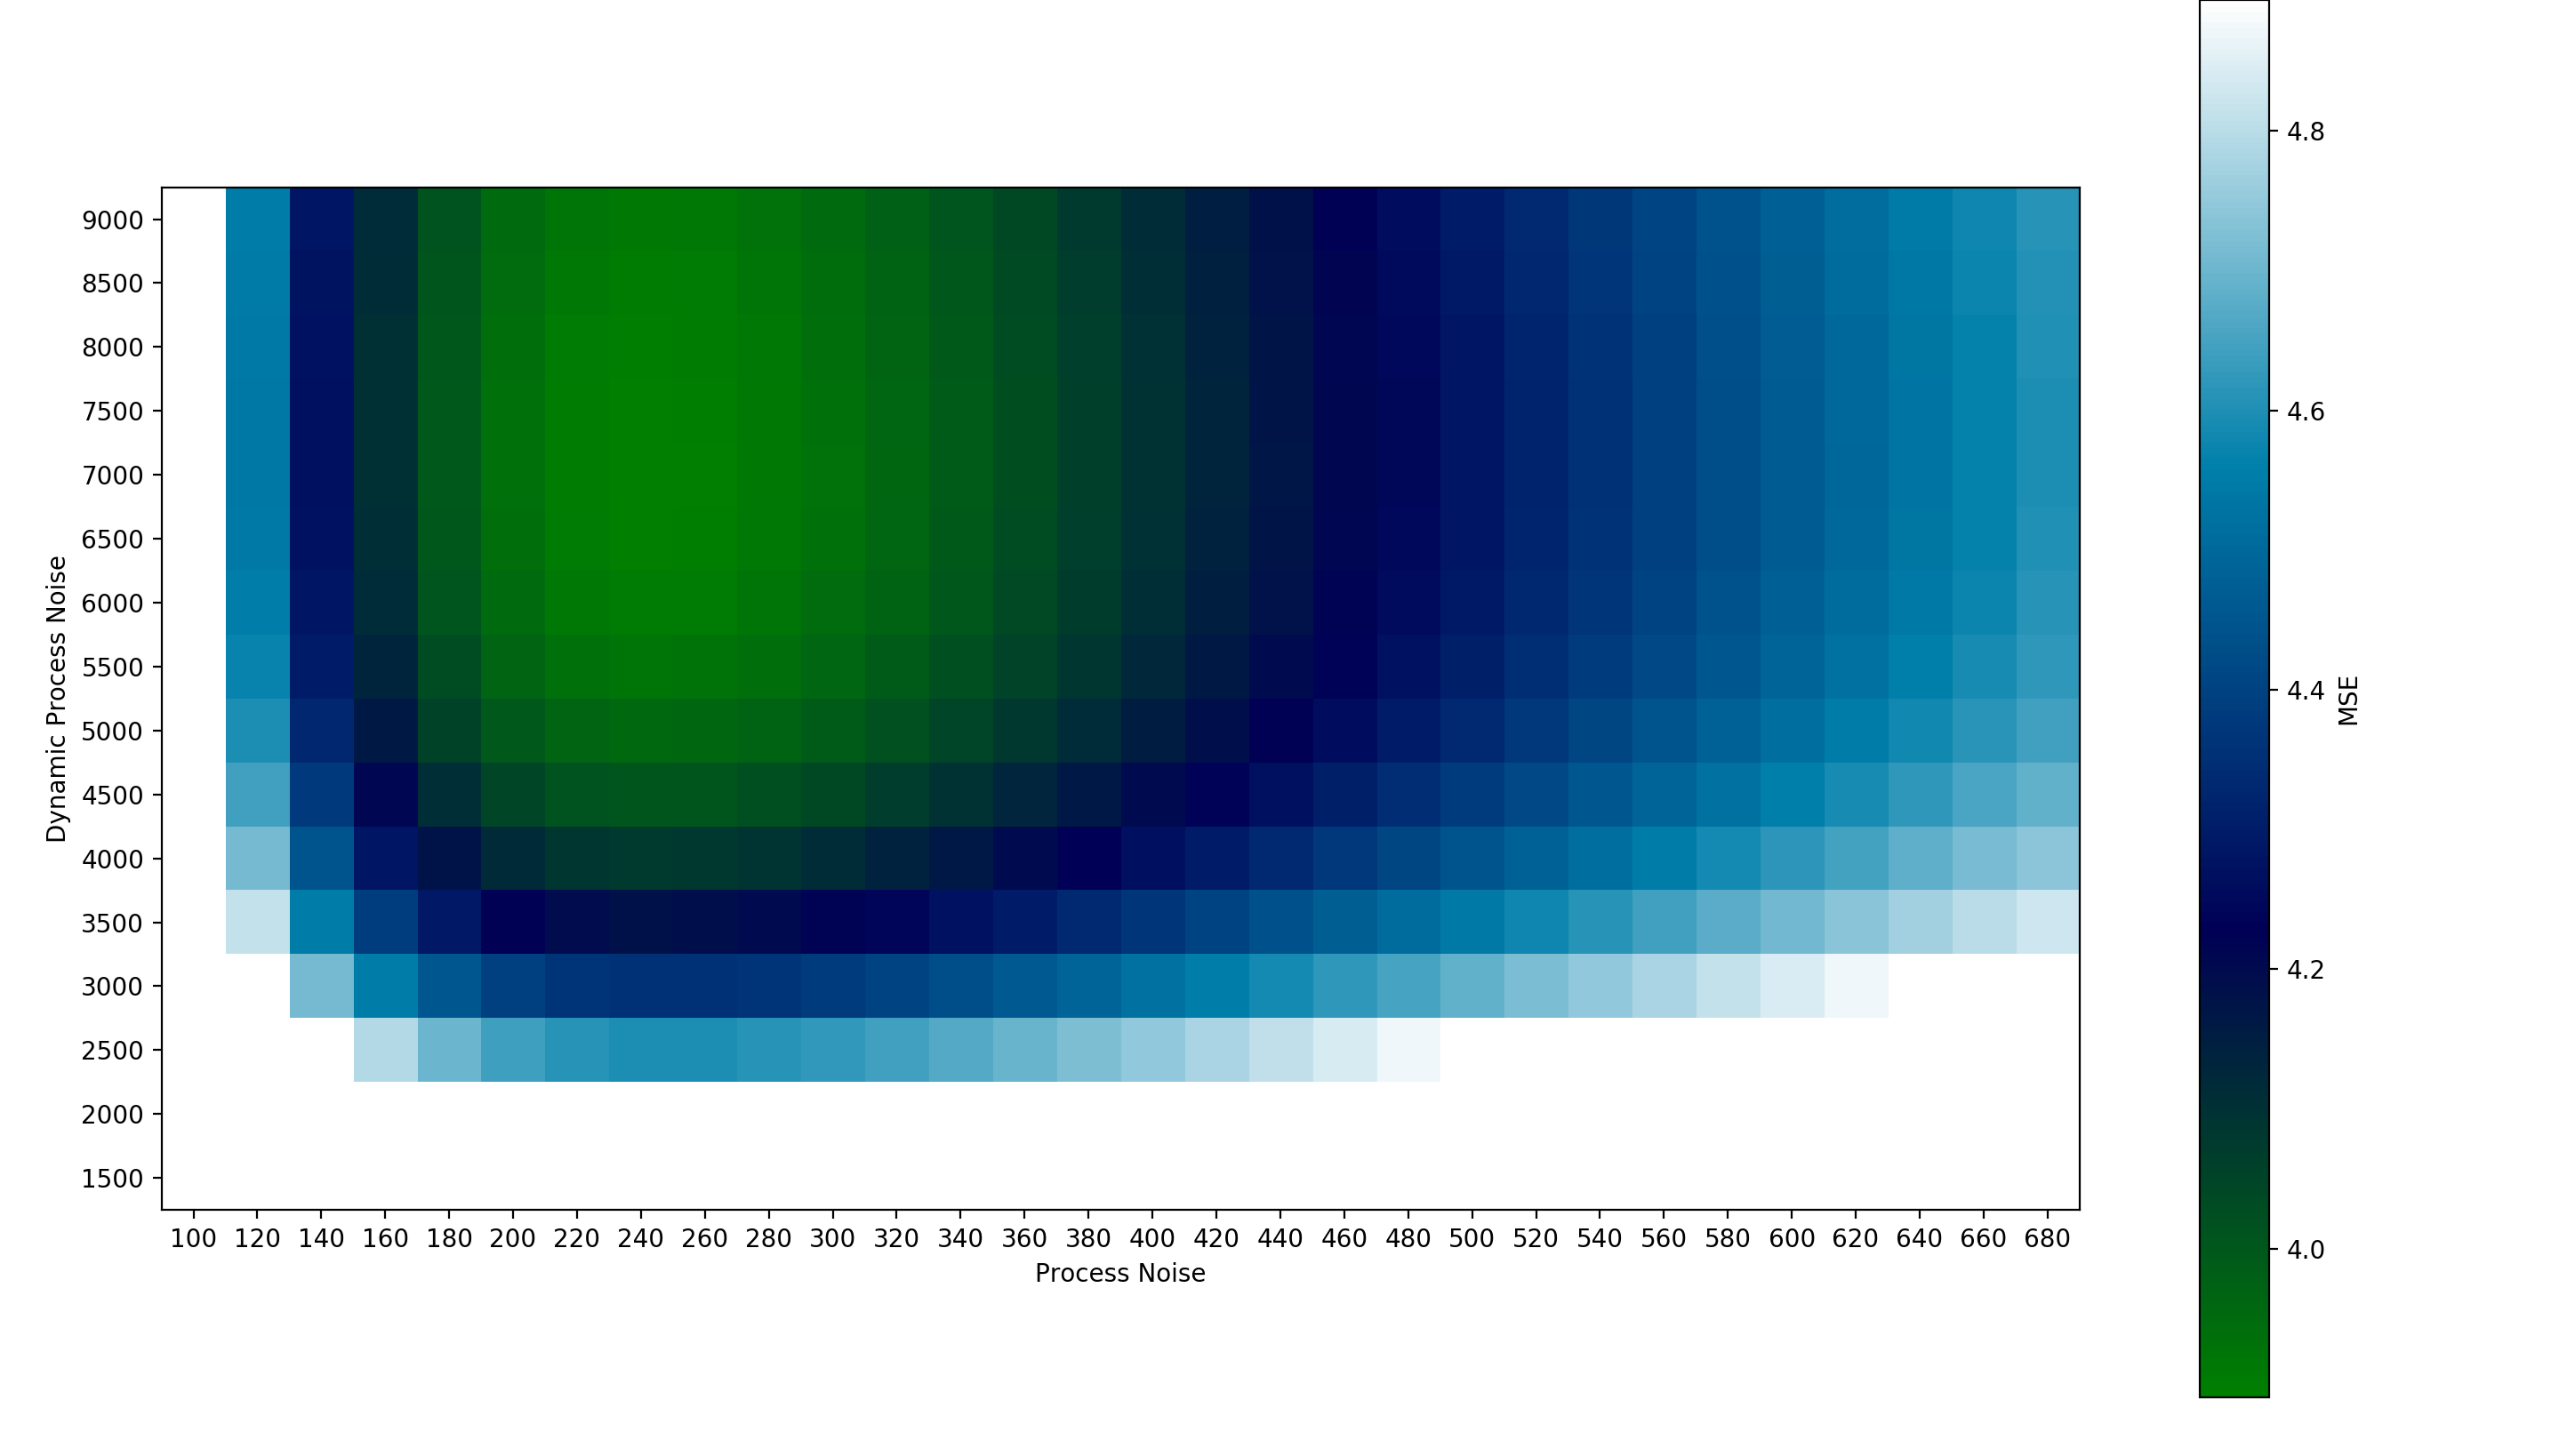
\includegraphics[width=0.68\textwidth]{dynamic_pn.png}}
    \caption{Simulation for optimal Q-Parameters}
    \label{fig:dyn-sim}
\end{figure}

The figure shows the two different $Q$ parameters for the two different operating modes: normal or proximity to cushion. 
The color scale represents the achieved MSE with this parametrization: green means better.
There is clearly a sweetspot for the optimal parametrization, which we chose to parametrize the filter with.
Although the optimal area continues further up the ordinate, it does not make sense to look for optimal parametrization there
because increasing these values would mean to approach the behavior of the sensor what wouldn't be beneficial.
As you can see the general process noise is much lower than the dynamic process noise.
This tells us, that the filter has to trust the sensor data more in those edge cases, but can rely on predictions after it hit the cushion.

\subsection{Smart Filter} \label{smart-filter}

In addition to the previous section we developed another improvement. In this case it can be assumed that the angle of incidence is equal to angle of reflection. 
With this assumption we can now implement the reflection with a single vector-multiplication expression. 

Assuming that we have a velocity vector pointing in the direction of $x$ and $y$, the operation to mirror on the x-axis is as in \cref{eq5}:

\begin{equation} 
    \label{eq5}
    \vec{v}_{mirror} = 
    \left(\!
    \begin{array}{c}
      v_x \\
      v_y
    \end{array}
    \!\right) \cdot
    \left(\!
    \begin{array}{c}
        -1 \\
        1
    \end{array}
    \!\right)
\end{equation}

As in the previous section this operation can be performed, when the ball hits the cushion.

Now the filter needs more information about the environment. We have to define the position of each cushion and the direction of each cushion to be able to calculate the correct reflection angle.

\section{Evaluation}

\subsection{Filter performance comparison} \label{perf-comp}

We developed a simulation, where we could test different parameters and scenarios to get reproducible results. 
We also used this simulation to determine the optimal value for the process noise in \cref{dynamic-q}. The results are shown in \cref{fig:sim-results}:

\begin{figure}[H]
    \centering
    \fbox{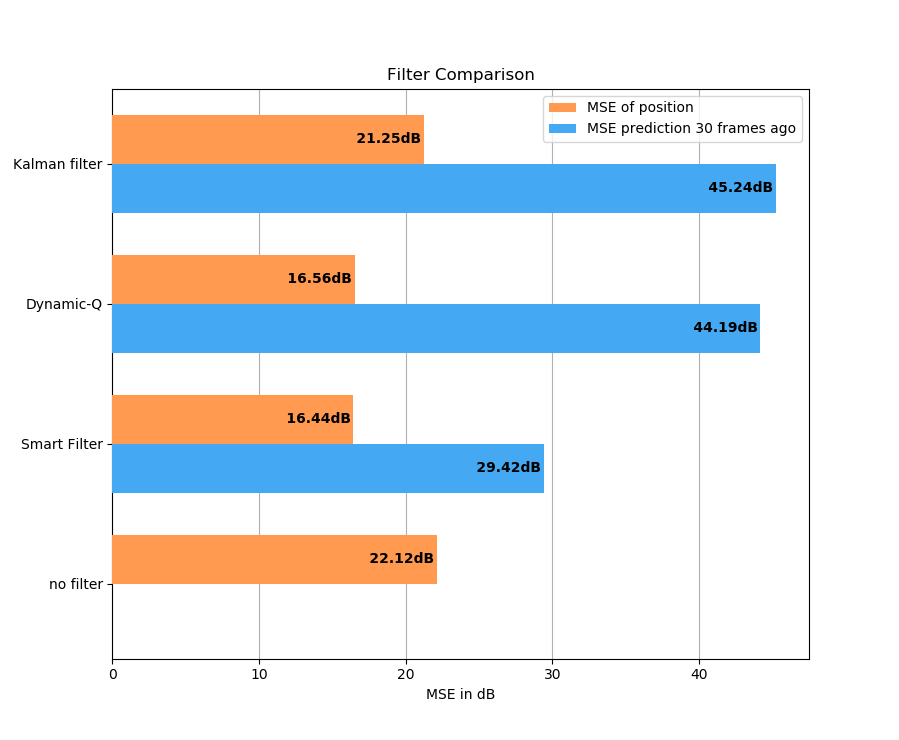
\includegraphics[width=0.68\textwidth]{filter_comparison_horizontal2.PNG}}
    \caption{Performance of different filter implementations}
    \label{fig:sim-results}
\end{figure}

The orange bar represents the quality of the filter output against the ground truth of the current position. 
The blue bar shows how much the prediction 30 frames in the future deviated from the ground truth.
You can see that the standard Kalman filter minimally improves the tracking compared to the bare sensor.
The improvement in tracking with the Dynamic-Q filter is as good as with the Smart filter.
But the prediction with the Smart filter is much better.

\begin{figure}[H]
    \centering
    \fbox{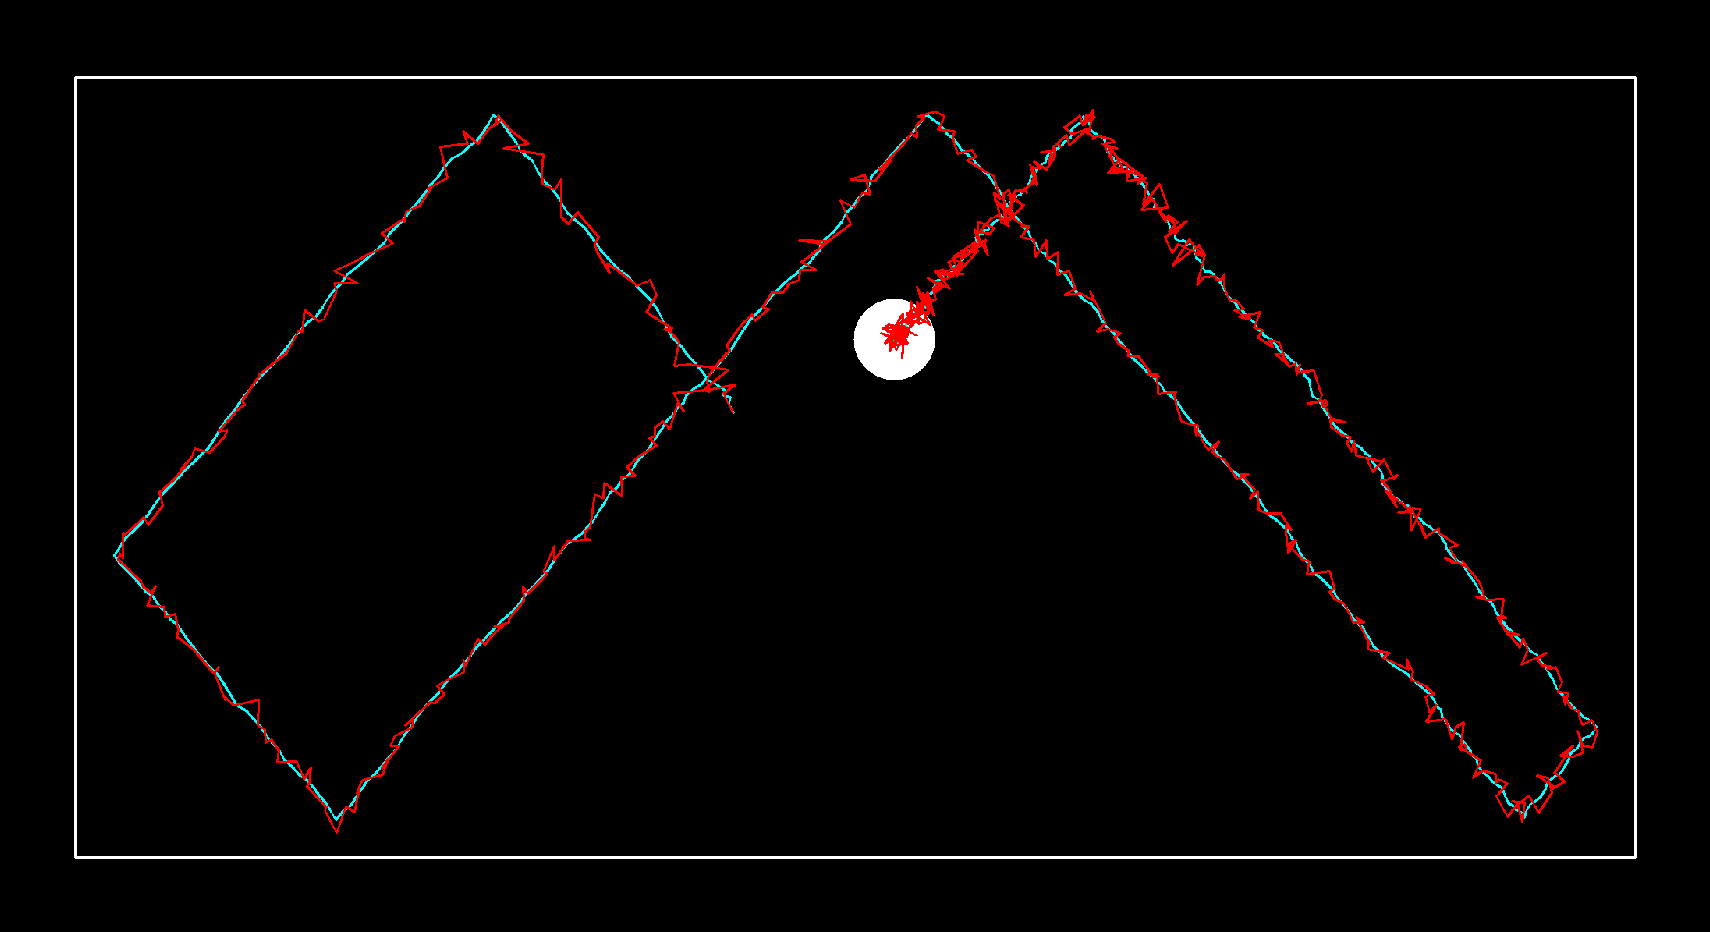
\includegraphics[width=0.68\textwidth]{smart_vs_noise.png}}
    \caption{Simulation with Smart Filter and sensor data}
    \label{fig:smart-vs-sensor}
\end{figure}

In \cref{fig:smart-vs-sensor} you can see the tracking path of the Smart filter (blue) and the senor data (red).
The sensor data is very noised and with the smart filter the tracking gains a lot of improvement.

Another impact the vector mirroring has is shown in \cref{fig:deviation-noise} on the time scale:

\begin{figure}[H]
    \centering
    \fbox{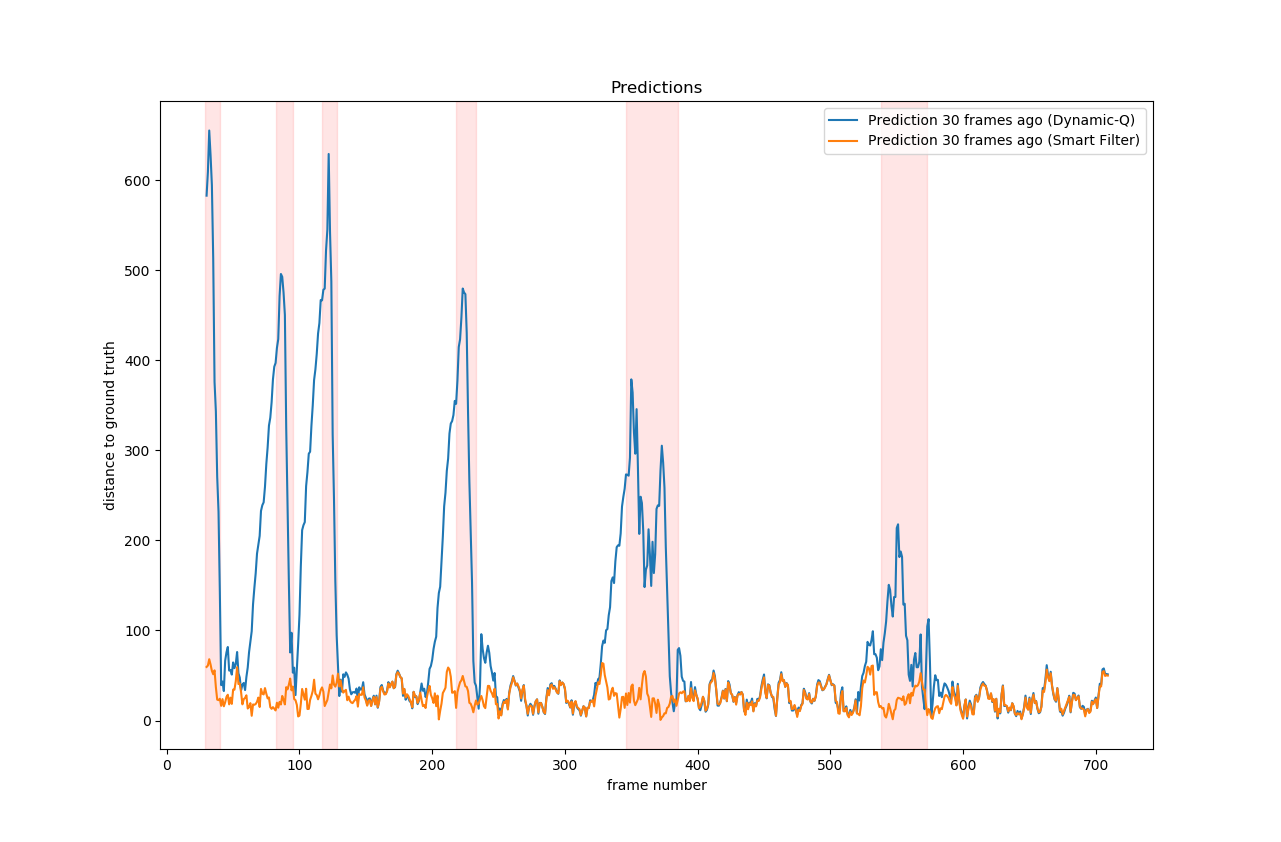
\includegraphics[width=0.68\textwidth]{prediction_dyn_smart_time2.PNG}}
    \caption{Performance of different filter implementations}
    \label{fig:deviation-noise}
\end{figure}

This figure represents the distance to ground truth over time for the prediction 30 frames into the future. 
The red areas are where the ball is close to the cushion. 
Although the dynamic-q enhancement (blue line) mitigates the overshoot problem, the prediction error rises quickly since the prediction accuracy degrades with a higher process noise.
The smart implementation however delivers constant accuracy regardless of any edge cases.

\subsection{Simulations}

We simulated the Smart filter with different technical parameters to examine its performance for predicting values 15, 30 or 60 frames in the future.
Displayed is the MSE of the prediction compared to the ground truth.

\subsubsection{Sampling}

The first simulation altered the sampling-rate. In a real-world scenario this would be the frame rate of the camera.

\begin{figure}[H]
    \centering
    \fbox{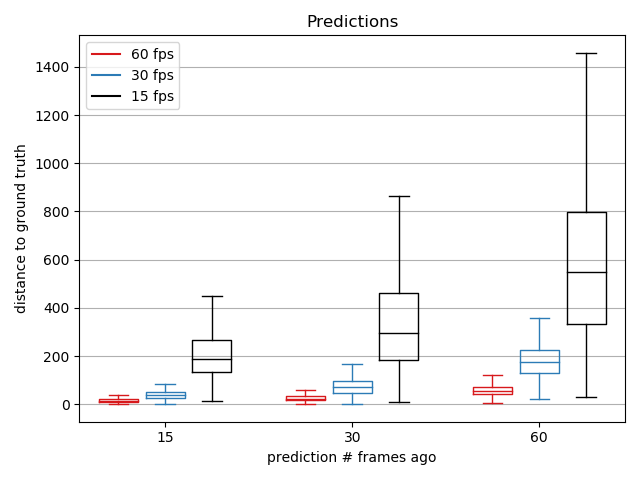
\includegraphics[width=0.68\textwidth]{fps_boxplot2.PNG}}
    \caption{Impact of framerates on prediction accuracy}
    \label{fig:framerate10}
\end{figure}

The sample rate has a certain impact on the quality of the prediction. However the the difference between 30 and 60 frames is not as big as between 10 and 30. 
This depends greatly on the initial velocity of the ball. Since the most cameras support framerates of at least 30fps, this performance is sufficient.

\subsubsection{Noise}

The second simulation altered the amount of noise on the measurement and how the filter is able to cope with bad input data.

\begin{figure}[H]
    \centering
    \fbox{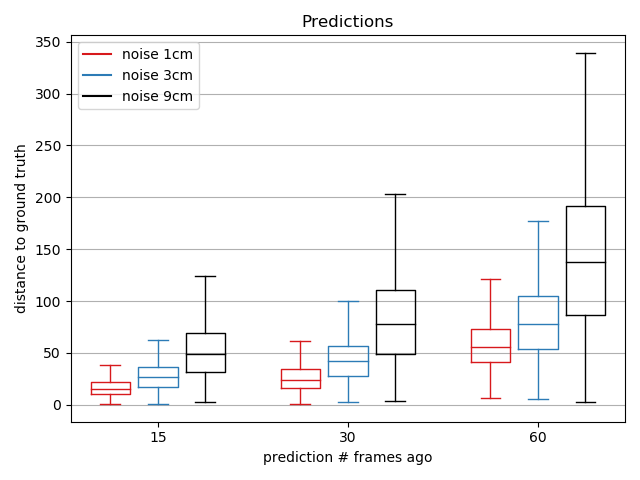
\includegraphics[width=0.68\textwidth]{noise_boxplot2.PNG}}
    \caption{Impact of sensor noise on prediction accuracy}
    \label{fig:noise2}
\end{figure}

Although the amount of noise increased fivefold, the median stays within the same magnitude of error compared to less noisy samples. The min and max values of deviation however change greatly on magnitude.
This is a good indicator that the filter is actually able to work with worse measurements than we used in our simulation and is still able to produce reasonably accurate predictions well into the future.

\subsubsection{Velocity}

Lastly we tested the impact of different starting velocities on the distance, which the ball rolls between the sample periods and how this affects the performance:

\begin{figure}[H]
    \centering
    \fbox{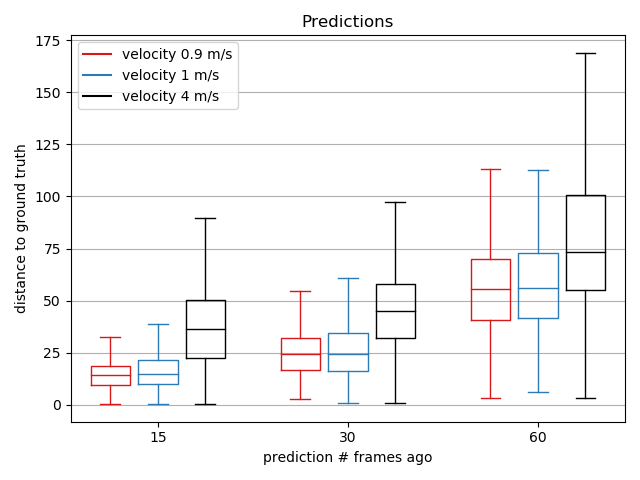
\includegraphics[width=0.68\textwidth]{velocity_boxplot2.PNG}}
    \caption{Impact of start velocities on prediction accuracy}
    \label{fig:velocity300}
\end{figure}

It shows that the starting velocity has barely any effect. 
This is what we expected since the sample rate is high enough to provide sufficient data. 
We also simulated different configurations in order to achieve the highest accuracy possible.

\subsection{Results with real footage}

After evaluating that our filter works well within the simulation, we tested it on real footage. 
It performed as expected and gave reasonably good predictions.

However, because of deviations in the tracking algorithm such determining the exact center of the ball and changing noise levels in the measurement, 
the filter performance is inferior to the simulation. Also the reflection-angle on the cushion was mathematically perfect in the simulation
but can vary by small margins in a real scenario.

\begin{figure}[H]
    \centering
    \fbox{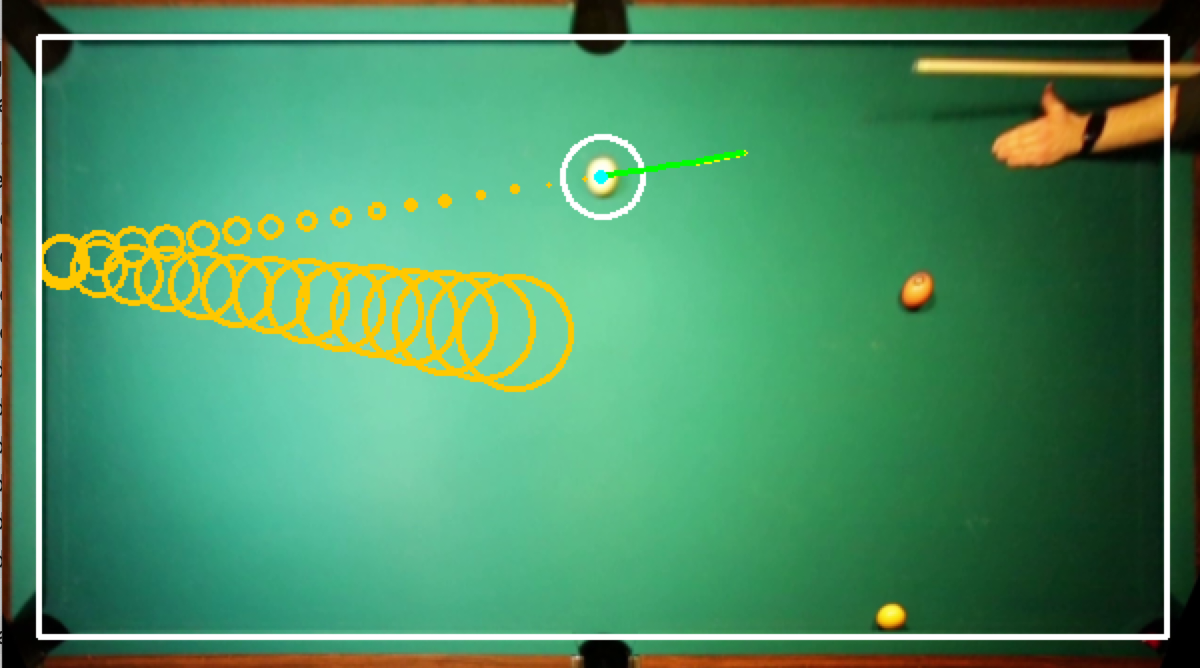
\includegraphics[width=0.68\textwidth]{pool_real.PNG}}
    \caption{Filter test on real footage}
    \label{fig:realfootage}
\end{figure}

Apart from the simulation we did not have data for the ground truth in this case. 
The quality of the filter can solely be measured by the quality of its prediction.

\section{Improvements}

An inherent problem with the nature of discrete values is that there are no reliable values in between to sample points. 
Although it is reasonable to assume that especially in linear cases the behavior between two sample points can interpolated, 
it is more complicated in this case due to the edge cases.

\begin{figure}[H]
    \centering
    \fbox{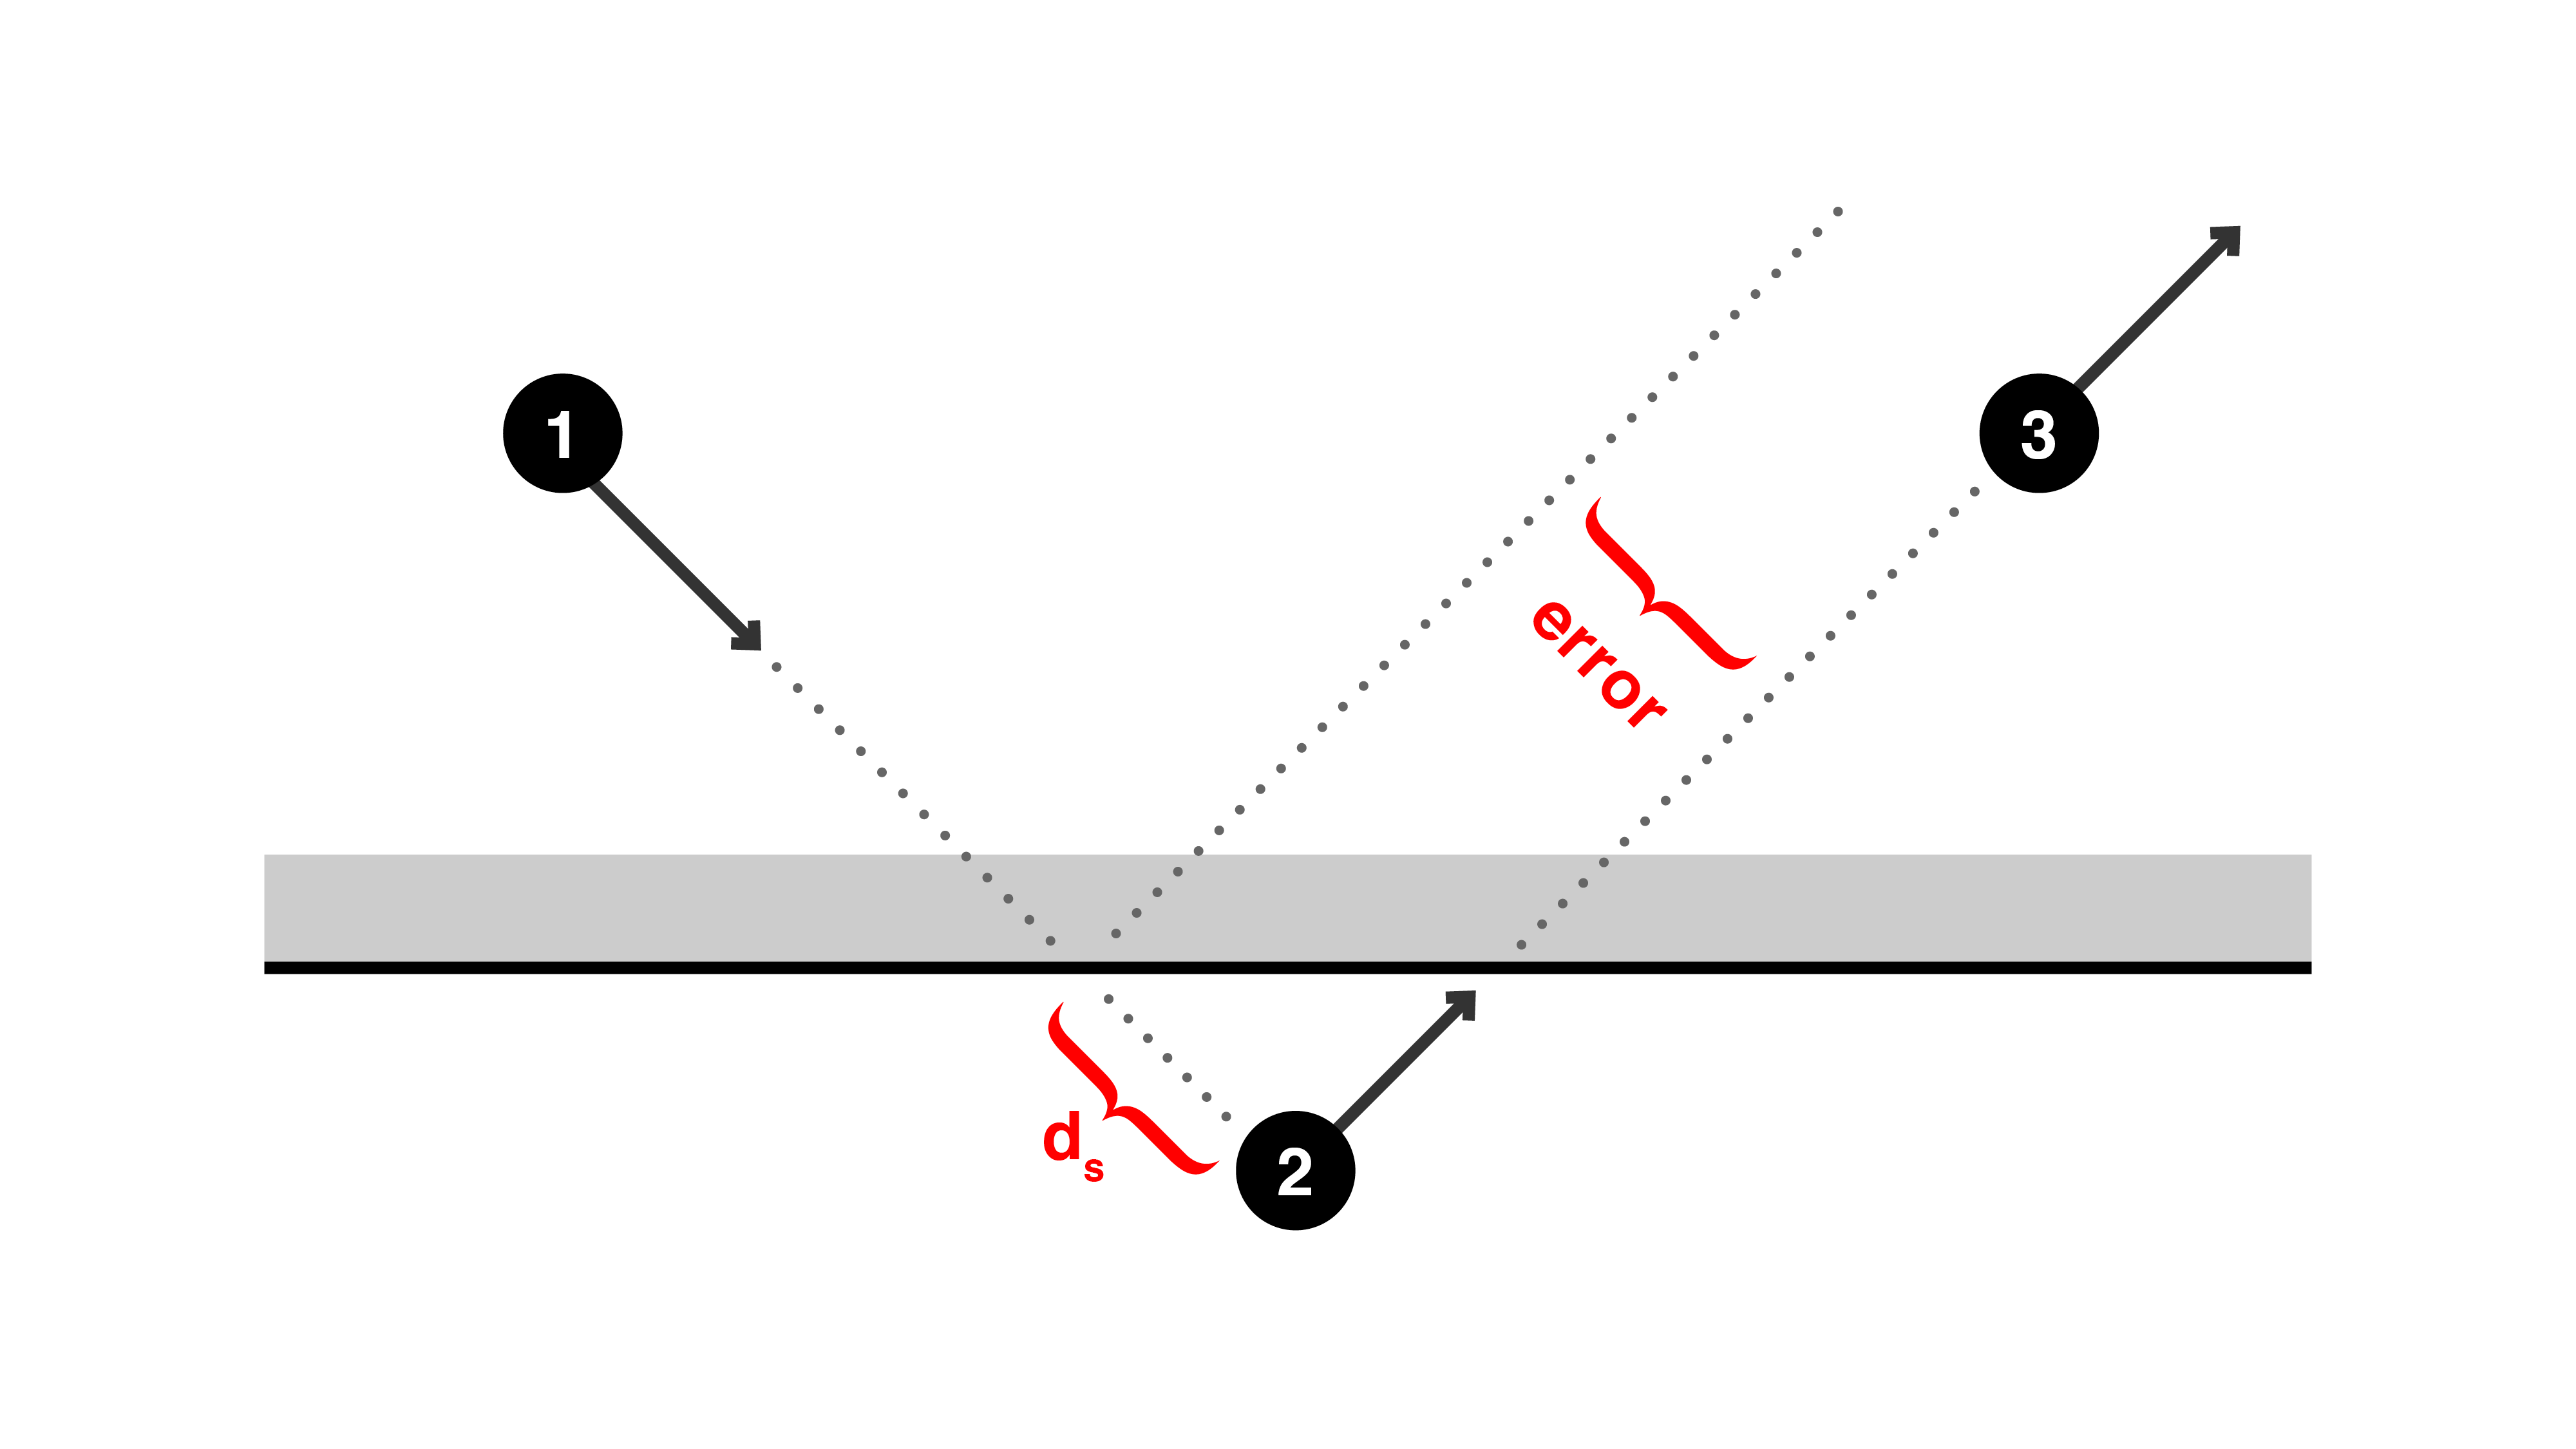
\includegraphics[width=0.68\textwidth]{prediction_error.PNG}}
    \caption{Ball hits cushion between two sample points}
    \label{fig:edge-case}
\end{figure}

As seen on \cref{fig:edge-case} the collision between the ball and the cushion is happens between sample 1 and 2. 
The filter detects this and turns the velocity vector as described in \cref{smart-filter}.
By the time of sample 3 the vector points in the right direction but with a offset. The correct solution however is shown in \cref{fig:edge-case-sol}:
The overshoot of sample 2 is corrected and mirrored on the point of collision, which affects the following samples. 
This will likely have a large positive impact on prediction accuracy as well as filter error.

\begin{figure}[H]
    \centering
    \fbox{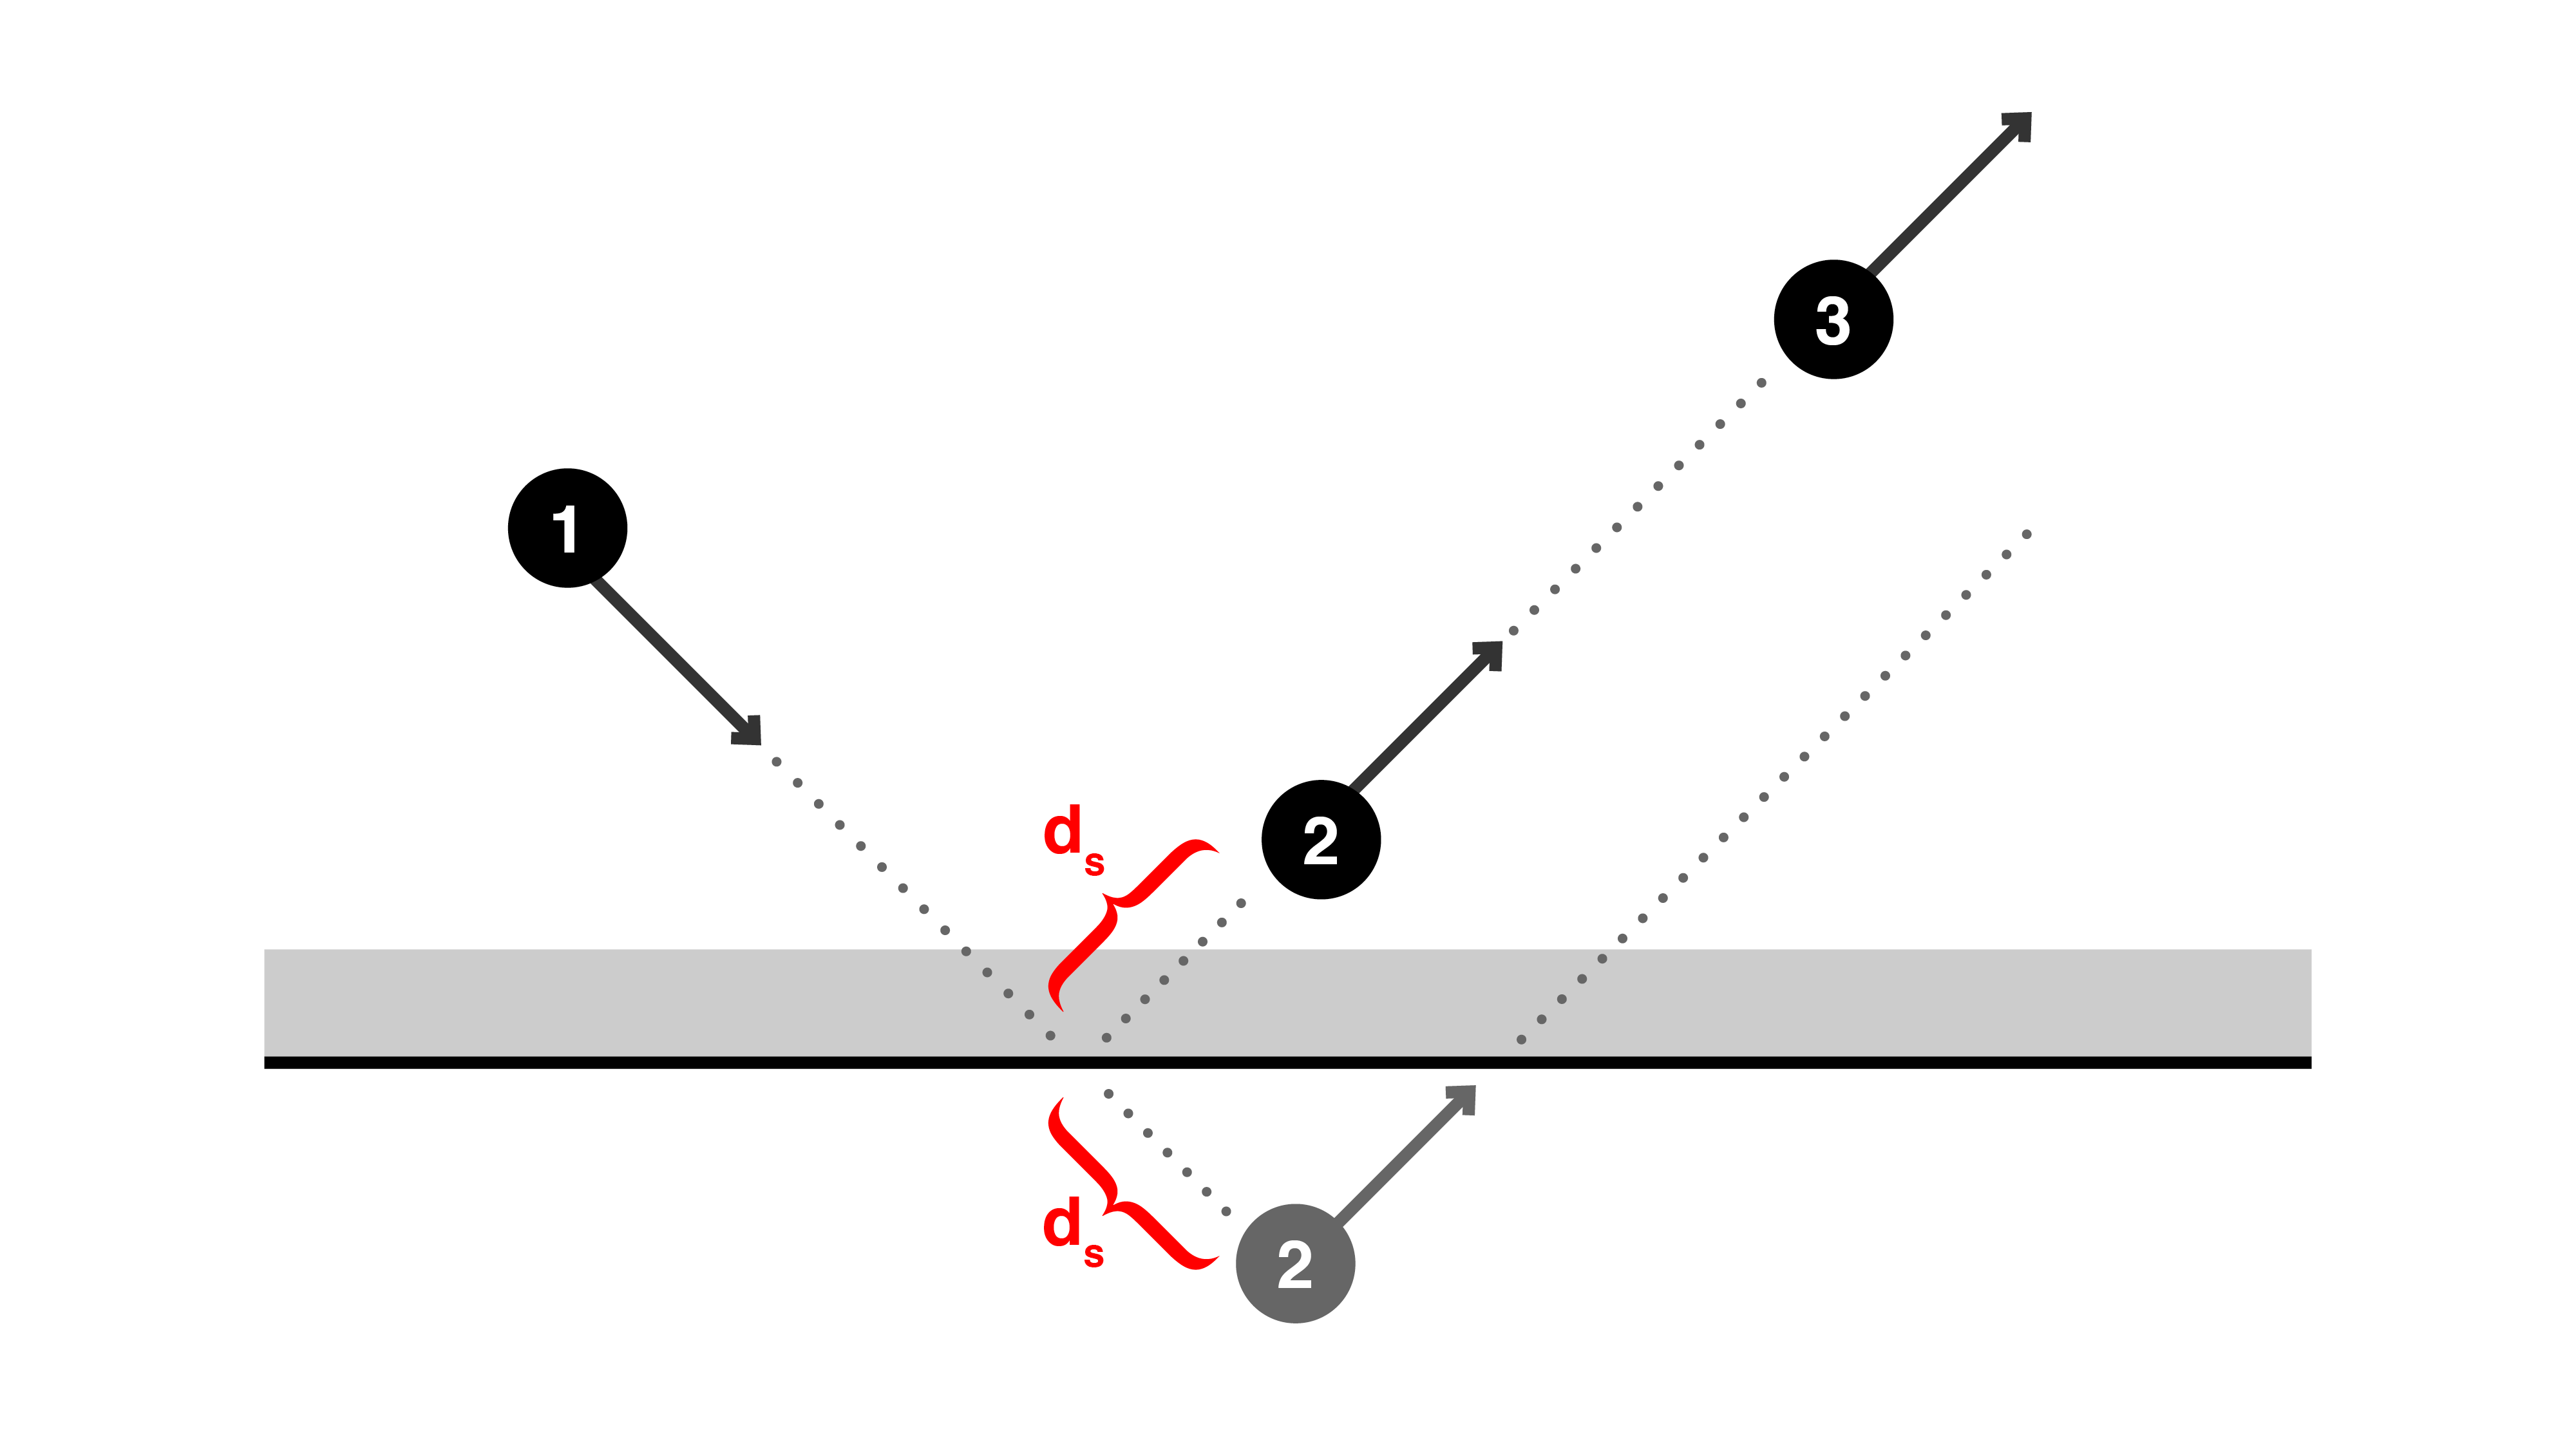
\includegraphics[width=0.68\textwidth]{prediction_correction.PNG}}
    \caption{Collision correction}
    \label{fig:edge-case-sol}
\end{figure}

Therefore it is a good starting point for further development.

\section{Conclusion} 

We found two solutions to improve the tracking of the billiard balls by extending the Kalman filter.
The first solution is to raise the process noise in critical areas to give the sensor data more weight in the calculation of the prediction.
This solution however gives false predictions, because the algorithm does not know how it has to adapt in critical situations and just blindly trusts the sensor data.

The second solution calculates exactly the behavior in the edge cases, which results in robust tracking and trustful predictions. But you have to feed information about the environment to the filter.
This is in a basic environment like a billiard game fairly easy but in a more advanced use case not trivial.


\section{Acknowledgement}

We would like to thank Prof. Edeler for his input during the lecture which really helped to further develop the idea.

\clearpage

\bibliography{references} 
\bibliographystyle{ieeetr}

\end{document}